\documentclass[10pt]{beamer}

\usetheme[progressbar=frametitle]{metropolis}
\usepackage{appendixnumberbeamer}

\usepackage{booktabs}
\usepackage[scale=2]{ccicons}

\usepackage{pgfplots}
\usepgfplotslibrary{dateplot}

\usepackage{xspace}
\newcommand{\themename}{\textbf{\textsc{metropolis}}\xspace}

\usepackage{caption}
%\usepackage{gensymb}
\usepackage{ulem}
\usepackage{subcaption}
\usepackage[french]{babel}
\usepackage{csquotes}
\usepackage[backend=biber,style=authoryear,citestyle=authoryear]{biblatex}

\DeclareCaptionLabelFormat{underlcap}{\uline{#1 #2}}
\DeclareCaptionLabelSeparator{underlcap}{~}
\DeclareCaptionTextFormat{underlcap}{\expandafter\uline\expandafter{\expandafter#1}}

\captionsetup[figure]{%
   labelformat=underlcap,labelseparator=underlcap,textformat=underlcap}
   
\newcommand\Wider[2][3em]{%
\makebox[\linewidth][c]{%
  \begin{minipage}{\dimexpr\textwidth+#1\relax}
  \raggedright#2
  \end{minipage}%
  }%
}

\makeatletter
\setlength{\metropolis@progressinheadfoot@linewidth}{1.7pt}
\setlength{\metropolis@titleseparator@linewidth}{1.7pt}
\setlength{\metropolis@progressonsectionpage@linewidth}{1.7pt}

\definecolor{alizarin}{rgb}{0.1, 0.26, 0.82}
\definecolor{bazaar}{rgb}{0.63, 0.63, 0.8}

\setbeamercolor{progress bar}{fg=alizarin,bg=bazaar}

\AtBeginSection[]{
  \begin{frame}
  \vfill
  \centering
  \begin{beamercolorbox}[sep=8pt,center,shadow=true,rounded=true]{title}
    \usebeamerfont{title}\insertsectionhead\par%
  \end{beamercolorbox}
  \vfill
  \end{frame}
}

\addbibresource{/Applications/ZoteroBibs/Library.bib}

\title{Concours de l'école doctorale des Sciences de l'Environnement}
\subtitle{Candidat: Félix Langot}
\date{\today}
\author{\textit{UVSQ/Paris-Saclay - University of Bristol}}
\institute{}
% \titlegraphic{\vfill
\includegraphics[height=1.5cm]{Figures/logo.png}}
\begin{document}

\maketitle

\section*{Présentation du cursus}
\begin{frame}{\secname}
\Wider{
    \begin{itemize}
        \item \textbf{Baccalauréat S (2016):} 
        \begin{itemize}
            \item mention TB, mention européenne, spécialité mathématiques.
            \item 17.5 de moyenne générale dont 19/20 en mathématiques et 17/20 en physique
        \end{itemize} 
        \item \textbf{MSci Physics with Astrophysics (2020):} 
        \begin{itemize}
            \item Obtention du master avec 'Upper second class honours' (mention bien)
            \item 'commendation' pour le projet final de master (note > 16)
            \item Passage de plusieurs unités avec des notes '1st class' (mention très bien) dont l'unité \textit{Geophysical Fluid Dynamics}
        \end{itemize}
        \item \textbf{Master ECLAT (2021):} 
        \begin{itemize}
            \item Moyenne du premier semestre de 15.4/20
            \item 18/20 de moyenne dans les U.E. de modélisation
        \end{itemize}
    \end{itemize}
}
\end{frame}

\section*{Expérience de recherche}
\begin{frame}{\secname}
\Wider{  
  \begin{columns}
  \column{0.7\textwidth}
    \textbf{MSci Physics with Astrophysics:} 
    \begin{itemize}
      \item Mesure de la vitesse de l'expansion de l'Univers $H_0$ en utilisant des observations rayon X de galaxies lointaines et l'effet de Sunyaev-Zel'dovich
      \item Simulations d'allées de tourbillons de Karman avec la méthode Lattice-Boltzmann avec parallélisation des processus
    \end{itemize}
  \column{0.3\textwidth}
    \begin{figure}[hbtp]
      \centering
      \includegraphics[width=3.6cm]{/Users/felixlangot/Library/Mobile Documents/com~apple~CloudDocs/Work/IV. Year 4/Project/Assessed/Final Report/13491regions.png}
\end{figure}
\end{columns}
\begin{columns}
  \column{0.5\textwidth}
  \begin{figure}[hbtp]
    \centering
    \includegraphics[width=5cm]{/Users/felixlangot/Library/Mobile Documents/com~apple~CloudDocs/Work/IV. Year 4/Advanced Computing/Mini-Project/Figure:Gifs/stlRe65.png}
  \end{figure}
  \column{0.5\textwidth}
  \begin{figure}[hbtp]
    \centering
    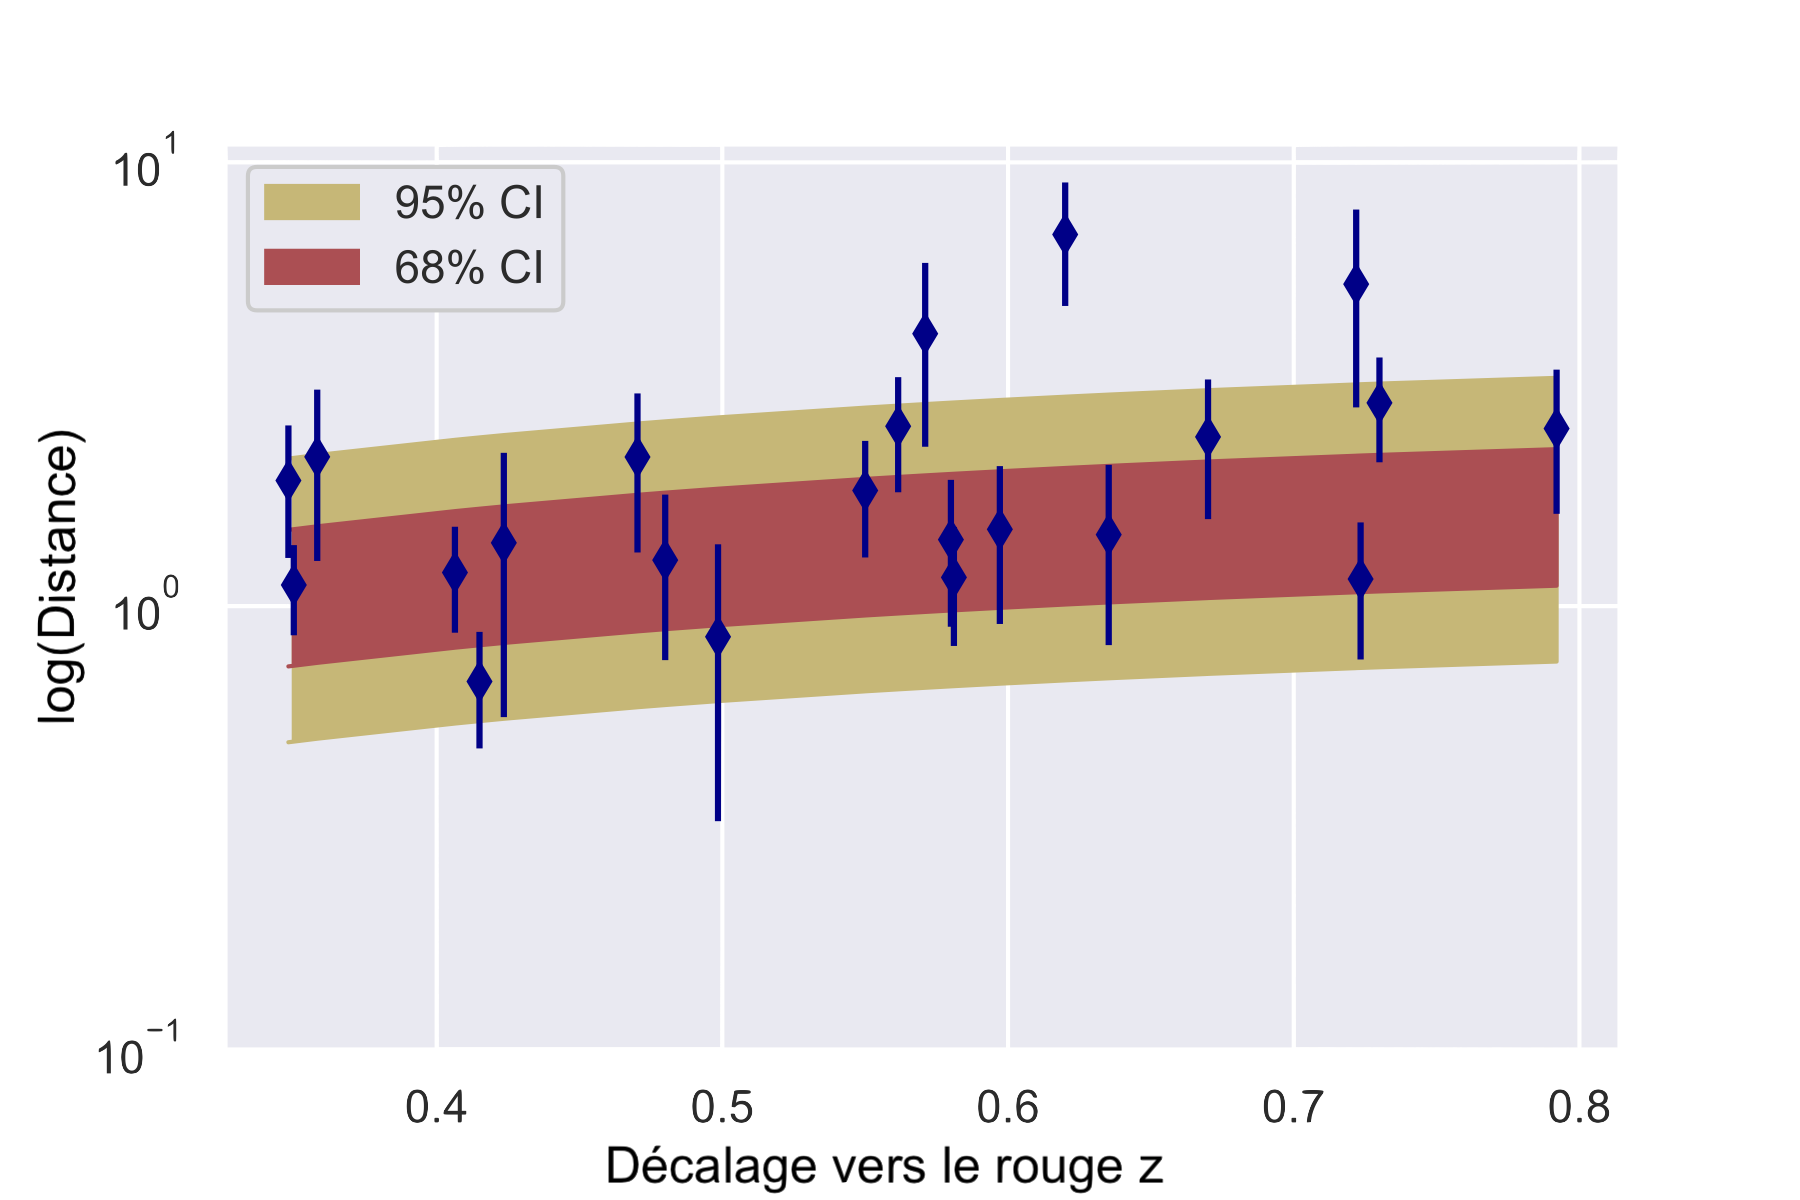
\includegraphics[width=5.5cm]{/Users/felixlangot/Library/Mobile Documents/com~apple~CloudDocs/Work/IV. Year 4/Project/Assessed/Final Report/HubbleGraphs/Logs.eps}
  \end{figure}
\end{columns}
}
\end{frame}

\begin{frame}{\secname}
\vspace{-0.3cm}
\Wider{
\begin{columns}
  \column{0.5\textwidth}
  \textbf{M2 ECLAT:}
  \begin{itemize}
    \item Stage au LMD: Impact de l'organisation de la convection profonde sur l'humidité de la troposphère \\
    $\rightarrow$ Publication des résultats prévue par Dr C. Risi
  \end{itemize}
  \column{0.5\textwidth}
  \hspace{-1cm}
  \begin{figure}[hbtp]
    \centering
    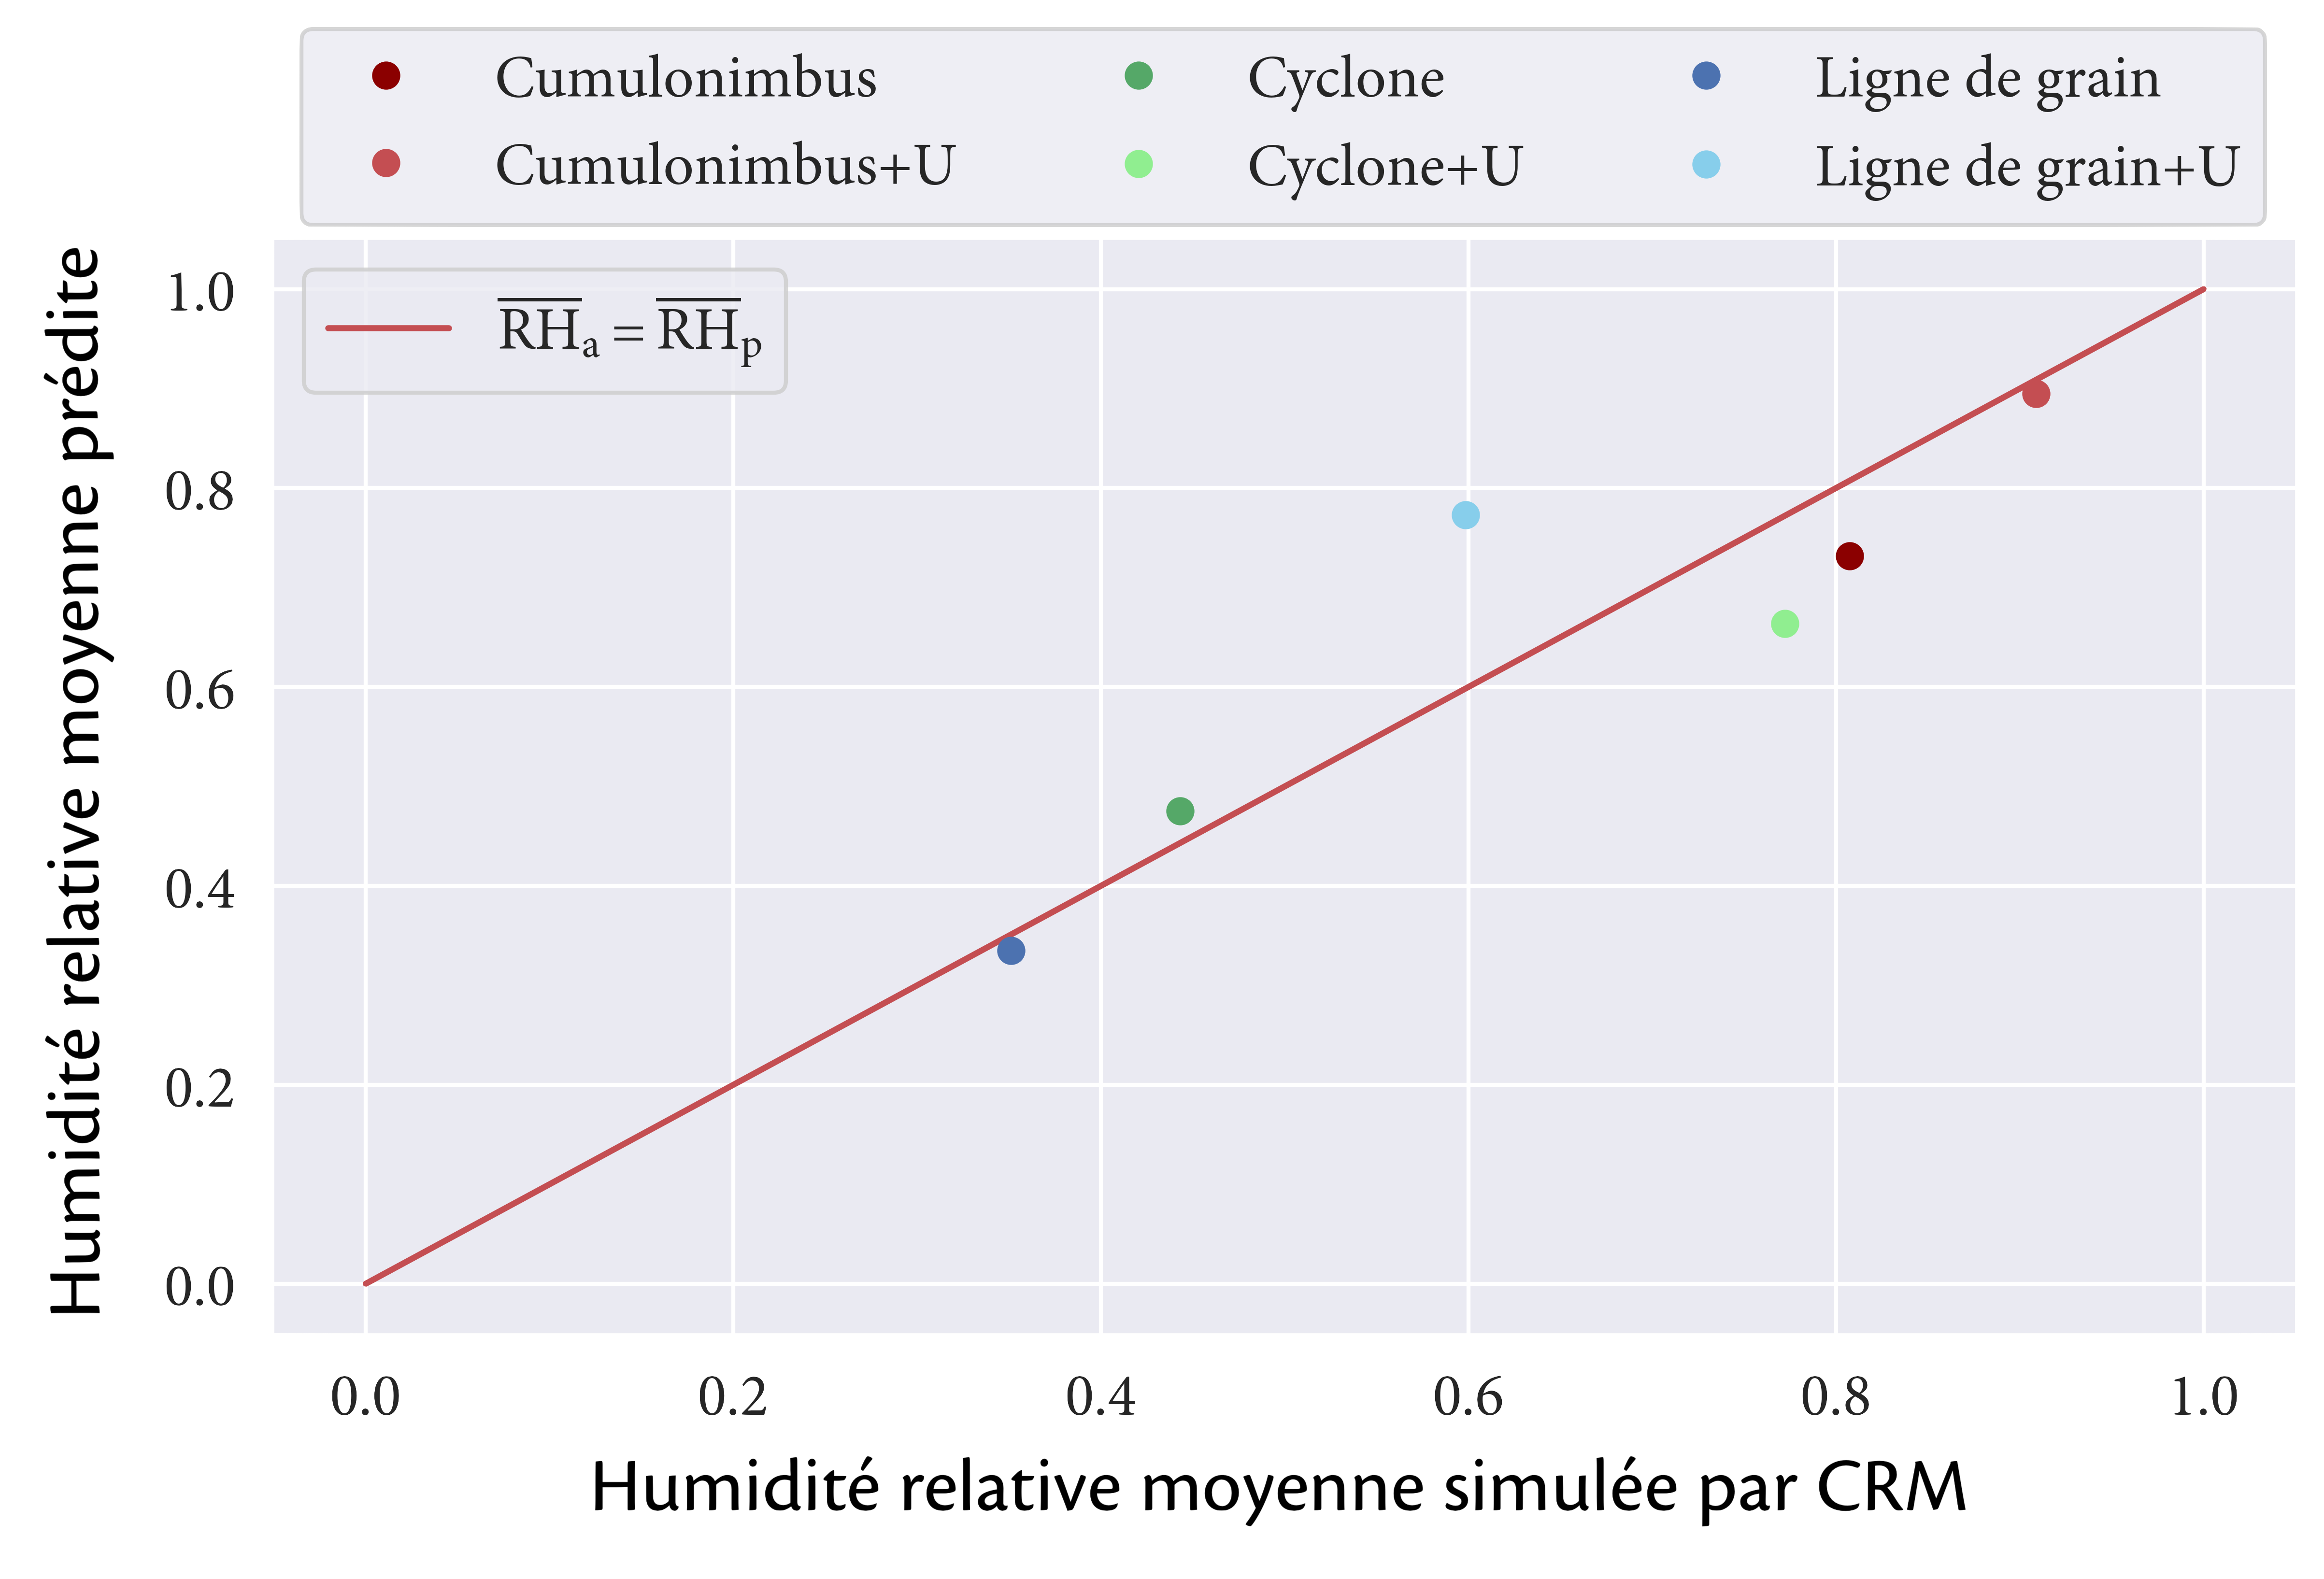
\includegraphics[width=5.5cm]{/Users/felixlangot/Stage/GitRepos/Codes/Figs/meanRHpvsRHa.png}
  \end{figure}
\end{columns}
\begin{figure}[hbtp]
  \centering
  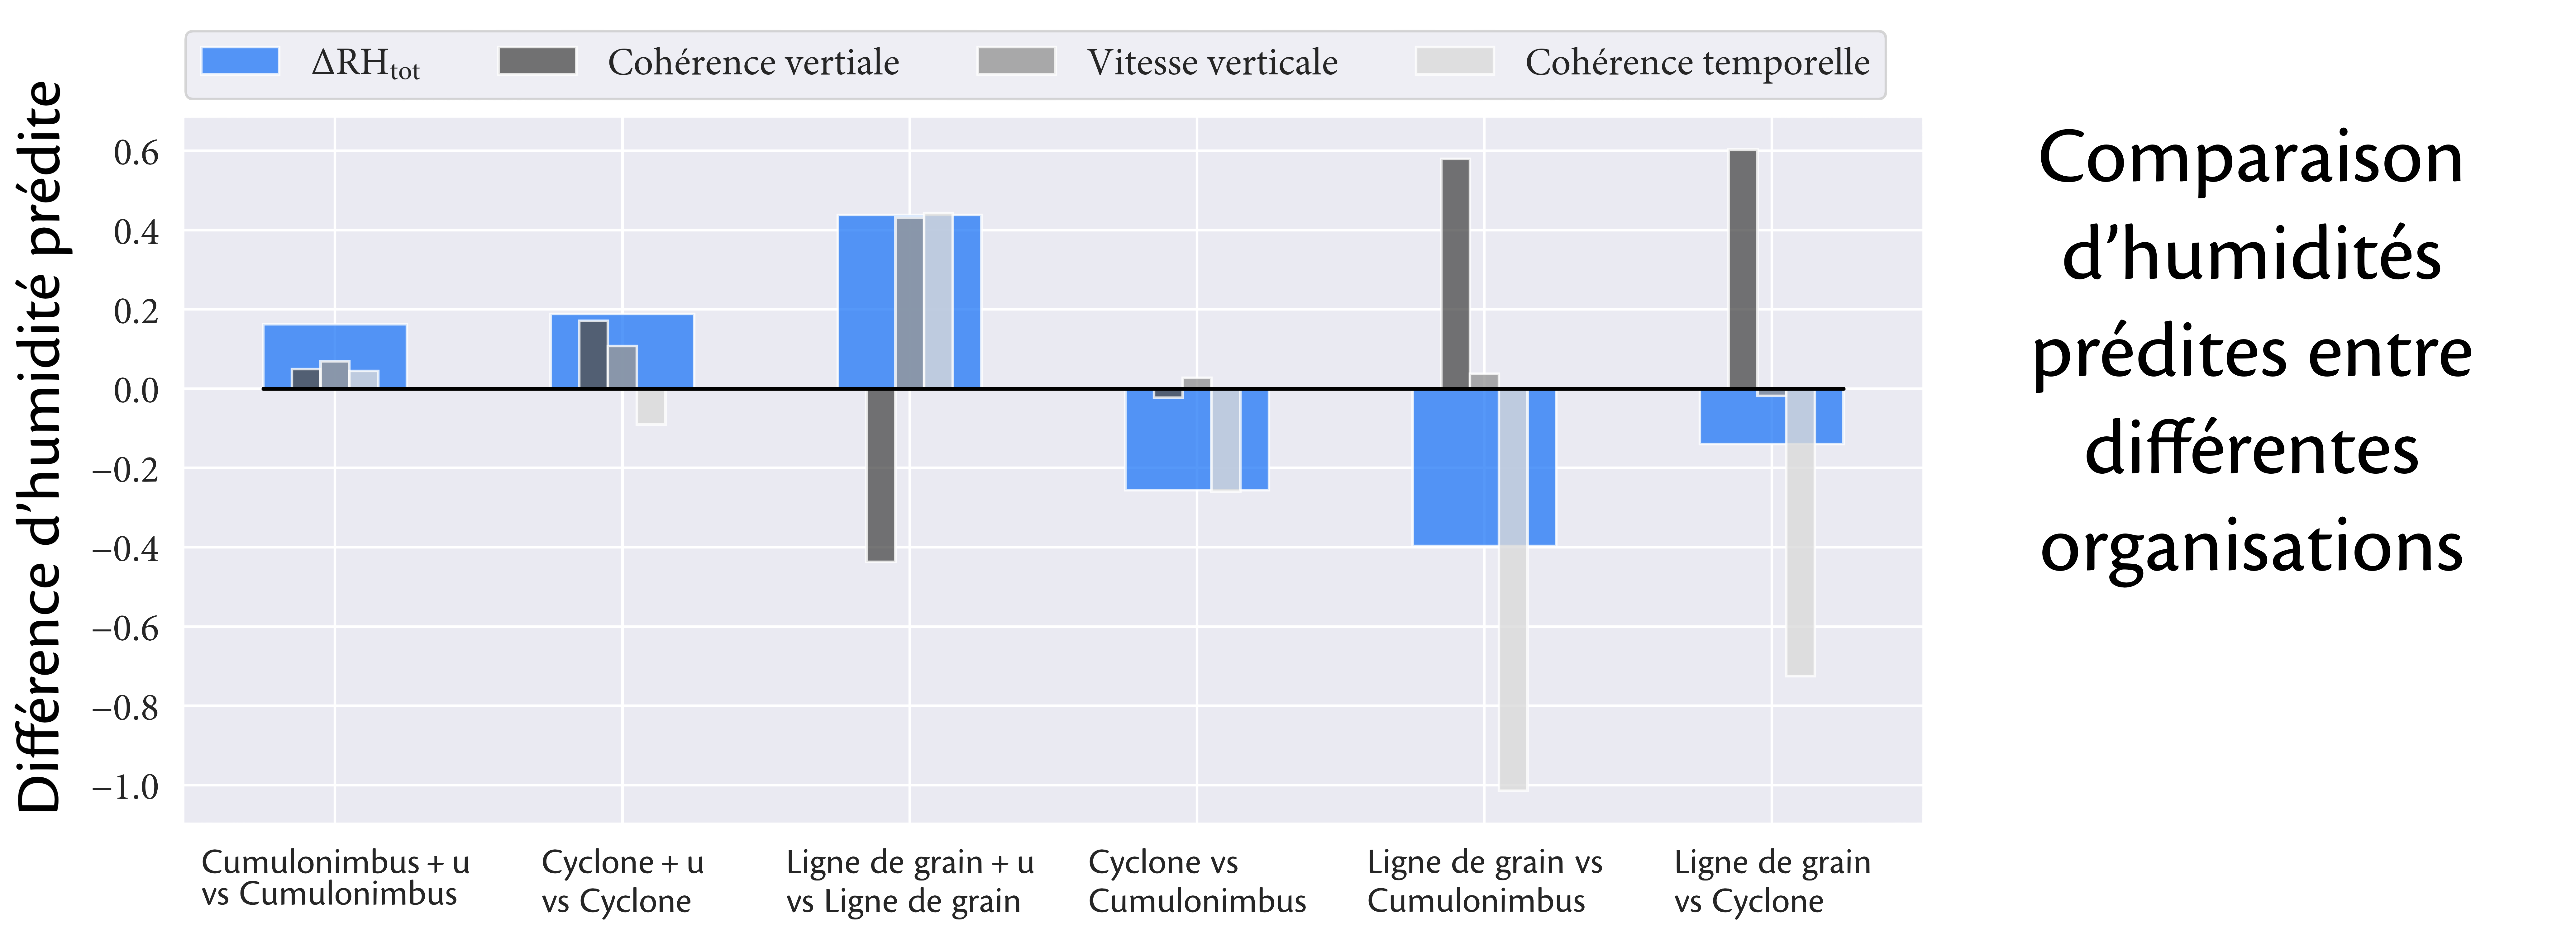
\includegraphics[width=10cm]{/Users/felixlangot/Stage/GitRepos/Codes/Figs/AllComps.png}
\end{figure}
}
\end{frame}

\section*{Projet}
\begin{frame}{\secname}
\Wider{
\textbf{Contexte:}
\begin{itemize}
  \item Projections climatiques incertaines, principalement à cause des nuages de couche limite
  \item Efforts pour réduire cette incertitude en améliorant la compréhension des mécanismes de rétroaction des nuages bas
\end{itemize}
\textbf{But:}
\begin{itemize}
  \item Comprendre le rôle de l'organisation à méso-échelle de ces nuages sur leur rétroaction climatique: catégoriser les morphologies nuageuses, analyser leur sensibilité aux perturbations météorologiques \\
\end{itemize}
$\rightarrow$ Établir des contraintes sur l’amplitude de la rétroaction des nuages bas
\textbf{Moyens:}
\begin{itemize}
  \item Utilisation de l'apprentissage automatique pour catégoriser les morphologies
  \item Étude de la corrélation entre changements morphologiques et variations de la dynamique de couche limite par observation satellites.
  \item 
\end{itemize}
% Dans un second temps, l’étudiant(e) quantifiera les co-variations entre changements morphologiques nuageux et variations de la dynamique de couche limite (hauteur, température, flux de surface) fournies par observations et réanalyses. Appliquer cette classification aux longues séries d’observations satellite disponibles permettra de détecter la sensibilité morphologique des nuages aux variations naturelles (Bony et. al, 20) et d’explorer les processus générant ces modifications. Enfin, l’étudiant(e) aura la possibilité d’étendre cette analyse par une comparaison aux simulations haute-résolution, par la réalisation de simulations résolvant les processus de fine échelle (Brient et. al, 19) et/ou par l’établissement de modèles analytiques encapsulant les principaux mécanismes de rétroaction nuageuse identifiés par l’analyse observationnelle.
}
\end{frame}

\end{document}
